\documentclass[12pt,a4paper]{article}

% Mathematics
\usepackage{amsmath,amssymb,amsthm,mathtools}

% Typography and layout
\usepackage[utf8]{inputenc}
\usepackage[T1]{fontenc}
\usepackage{lmodern}
\usepackage[margin=1in]{geometry}
\usepackage{setspace}
\onehalfspacing
\usepackage{titlesec}
\titleformat{\section}[block]{\normalsize\bfseries\centering}{\thesection.}{0.5em}{}
\titleformat{\subsection}[block]{\normalsize\itshape\centering}{\thesubsection.}{0.5em}{}

% Tables and figures
\usepackage{booktabs,array,multirow,float,tabularx}
\usepackage{graphicx}

% Colour and links
\usepackage[dvipsnames]{xcolor}
\usepackage[round,sort&compress]{natbib}
\usepackage{hyperref}
\hypersetup{colorlinks=true,linkcolor=blue!60!black,citecolor=blue!60!black,urlcolor=blue!60!black}

% Page numbering
\usepackage{lastpage}
\usepackage{fancyhdr}
\pagestyle{fancy}
\fancyhf{}
\rfoot{\thepage}
\renewcommand{\headrulewidth}{0pt}

% Theorem environments
\newtheorem{corollary}{Corollary}
\newtheorem{definition}{Definition}
\newtheorem{assumption}{Assumption}
\newtheorem{lemma}{Lemma}
\newtheorem{prediction}{Empirical Prediction}
\newtheorem*{remark}{Remark}

% Custom commands
\newcommand{\R}{\mathbb{R}}
\newcommand{\E}{\mathbb{E}}
\newcommand{\indic}{\mathbb{1}}
\newcommand{\btheta}{\boldsymbol{\theta}}
\newcommand{\bW}{\mathbf{W}}

\title{\large\textbf{Pricing Transition Credibility on Spatial Networks}\vspace{-0.5em}}
\author{\normalsize Jose Luis Resendiz\\[4pt] \small Smith School of Enterprise and the Environment, University of Oxford}
\date{\small\today}

\begin{document}
{\singlespacing\maketitle}

\begin{quotation}\small\singlespacing\noindent
\textbf{Abstract:} A single plant retirement transmits opposing shocks through spatial networks: negative contagion for fuel-similar peers and positive competitive benefit for geographic neighbours. Using plant-level data for 389 listed utilities worldwide, we develop and test a networked pricing framework that reveals a credibility gap in how markets process transition risk. Three findings emerge. First, portfolio sorts confirm a channel split of 11.48 percentage points ($t=14.00$) between geographic and fuel exposure quintiles, with spatial coefficients robust to Conley standard errors at 1,000 km. Second, voluntary retirement filings raise peer return volatility ($t=3.89$) without moving mean prices ($t\approx 0$), revealing a credibility gap: markets observe network exposure but cannot price its direction until binding policy intervenes. Third, emissions trading systems sharpen the stranding channel ($w^{\text{fuel}} \times \text{ETS}$, $t=-3.41$), while a geographic placebo is null ($t=0.64$), directly testing the model's prediction that policy credibility moderates the fuel penalty. In a horse race against ESG ratings, the spatial signal dominates ($t=-3.94$ vs.\ $t=-0.59$), and a composite Spatial Transition Score generates an out-of-sample portfolio spread of $-7.75\%$ ($t=-6.10$). These results suggest that transition risk assessment should incorporate the spatial network connecting firms, not merely the characteristics of individual firms.
\end{quotation}

%----------------------------------------------------------------------
\section{Introduction}\label{sec:intro}
%----------------------------------------------------------------------

When a coal plant retires, the stock prices of technologically similar utilities fall while those of geographically proximate utilities rise. The same physical event produces opposite-signed spillovers depending on how firms are connected through the spatial network. This finding has broad implications for how financial markets assess transition risk, because the dominant assessment tools operate at the firm level and miss the network dimension entirely. The scale of the challenge is large: meeting the 2$^\circ$C target requires leaving over 80 percent of coal reserves unextracted, concentrating stranded asset exposure in specific geographies, with up to \$24 trillion in global financial assets potentially at risk \citep{McGlade2015, Dietz2016}. Finance academics and practitioners broadly agree that markets underestimate this exposure, a difficulty compounded by deep Knightian uncertainty propagating across carbon dynamics, temperature dynamics, and damage functions simultaneously \citep{StroebelWurgler2021, Barnett2020}. The financial industry's response has been firm-level scoring: ESG ratings, implied temperature scores, and target validation frameworks. This approach suffers from well-documented limitations. Major rating providers disagree on basic assessments of the same company, with pairwise correlations as low as 38 percent \citep{Berg2022}. Even mandatory sustainability reporting fails to produce consistent data, because underlying incentives create strategic variation in what companies disclose \citep{Christensen2021}. Corporate climate targets frequently fail basic integrity criteria, and markets exhibit weak reactions when firms miss stated goals \citep{JiangKimLu2025}. Institutional investors overwhelmingly believe climate risks are financially material yet report lacking adequate tools to measure portfolio-level exposure \citep{Krueger2020}. The problem is not a shortage of data or disclosure mandates, but a conceptual gap: firm-level approaches cannot capture risks that originate in the network connecting firms.

This paper develops and tests a spatial network framework for pricing transition risk. We decompose the network linking power utilities into three independently constructed layers: fuel-mix similarity, geographic proximity, and regulatory proximity. A single physical restructuring shock (a plant retirement) propagates through these layers with opposing signs. The framework yields a testable credibility gap: when the direction of a network shock is ambiguous, markets should respond through volatility rather than directional returns; when binding policy resolves the ambiguity, prices should adjust. We test these predictions using plant-level geolocation data for 389 listed power utilities worldwide, covering 72,398 event-firm pairs around 179 first-mover retirement events.

Three principal findings emerge, each supported by multiple identification strategies.

First, the spatial network predicts transition returns with a clean channel split. A joint $F$-test rejects the null that all spatial coefficients are zero ($F=11.28$, $p=0.001$), and a formal difference test confirms the opposing-sign structure ($\beta_{\text{geo}} - \beta_{\text{fuel}} = 1.851$, $t=3.65$, $p=0.0003$). Portfolio sorts sharpen this result: the channel split between geographic and fuel quintile spreads is $+11.48$ percentage points ($t=14.00$), robust to Conley standard errors at 1,000 km.

Second, voluntary retirement filings (EIA-860) raise peer return volatility without moving mean prices (volatility $t=3.89$; CAR $t=-0.17$). This is the signature of a credibility gap. The opposing channels offset in expectation, leaving the mean return near zero while injecting uncertainty into exposed firms' cash flow distributions.

Third, emissions trading systems sharpen the stranding channel. The fuel-similarity interaction with ETS presence is strongly negative ($w^{\text{fuel}} \times \text{has\_ets} = -3.24$, $t=-3.41$, one-sided $p=0.0003$, as the model predicts $\beta_2 < 0$), while a geographic placebo is null ($t=0.64$). In a horse race with ESG scores, spatial exposure dominates ($t=-3.94$ vs.\ $t=-0.59$), and a composite Spatial Transition Score produces an out-of-sample portfolio spread of $-7.75\%$ ($t=-6.10$) in the post-2020 period.

The paper makes three contributions. First, to climate finance: we establish that transition risk is a network property, not merely a firm characteristic. The opposing-sign spatial structure means that firm-by-firm divestment campaigns can inadvertently subsidise neighbouring fossil assets through the geographic competitive channel ($\gamma_G > 0$), creating a paradox of isolated climate action. Second, to asset pricing: the opposing channels create a structural information friction that manifests as volatility without directional repricing, explaining why ambiguous transition signals fail to move prices. Only binding policy resolves this friction. Third, to practitioners: spatial exposure is measurable from public registries (GEM plant data, GPS coordinates, ETS membership), complements existing firm-level frameworks, and captures a network dimension currently absent from assessment tools.

Our work connects to several literatures. The network architecture draws on \citet{AcemogluCarvalhoOzdaglarTahbazSalehi2012} and \citet{Herskovic2018}, who establish that production network linkages are priced in equilibrium. The opposing-sign spatial structure formalises the contagion-versus-competition dichotomy of \citet{LangStulz1992} and \citet{JorionZhang2007}. The credibility gap builds on the policy uncertainty literature of \citet{PastorVeronesi2012} and the cheap-talk framework of \citet{CrawfordSobel1982}. The volatility evidence connects to \citet{Bloom2009} and \citet{KellyPastorVeronesi2016} on uncertainty resolution. Within climate finance, we complement the carbon premium of \citet{Bolton2021} and \citet{BoltonKacperczyk2023}, the carbon tail risk of \citet{IlhanSautnerVilkov2021}, and the network stress tests of \citet{Battiston2017} and \citet{Battiston2021}. The electricity sector as an empirical laboratory follows \citet{Cicala2022} and \citet{FabrizioRoseWolfram2007}, and the geographic identification strategy follows \citet{GrieserHadlockLeSageZekhnini2022} and \citet{PirinskyWang2006}.

The paper proceeds as follows. Section~\ref{sec:model} develops the theoretical framework and lays out the empirical strategy. Section~\ref{sec:results} presents results. Section~\ref{sec:discussion} discusses implications for transition risk assessment and policy. Section~\ref{sec:conclusion} concludes. Appendices provide channel definitions, derivations, robustness tables, and data construction details.

%----------------------------------------------------------------------
\section{Empirical Framework: Networked Pricing under Policy Uncertainty}\label{sec:model}
%----------------------------------------------------------------------

\subsection{Overview}

Industry-standard assessment tools, including ESG ratings, implied temperature scores, and TCFD-aligned disclosures, treat each firm in isolation, assuming markets can continuously and accurately price firm-level commitments. We propose a different framework: the \textbf{credibility gap} is fundamentally an information friction. Investors observe the physical network of power utilities and each firm's legacy asset exposure, but they cannot reliably assign a directional price to transition commitments until binding policy removes managerial and political discretion.

We frame transition risk as an asset-pricing problem on a multi-layered spatial network under regulatory uncertainty. This framework yields two core short-horizon insights. First, spatial transmission operates through distinct channels with opposing signs. Second, when the regulatory regime is uncertain, idiosyncratic shocks (e.g., plant-level retirements) act as noisy signals that increase return volatility without a clear directional mean. Conversely, binding phase-out laws partially resolve uncertainty, compress volatility, and generate negative returns proportional to firms' own fossil exposure.

\subsection{Environment and Networked Cash Flows}
%----------------------------------------------------------------------

Consider a continuum of listed power utilities $i \in [0,1]$. Firm $i$'s fundamental value is the expected present discounted value of its future cash flows, $V_i = \E[\Pi_i]$. Each firm is characterized by its \textbf{legacy asset intensity}, $\alpha_i \in [0,1]$, which measures reliance on fossil generation (e.g., coal share).

Firms are interconnected via a spatial network decomposed into three row-normalized adjacency matrices: geographic proximity ($\bW^{\text{geo}}$), fuel-mix similarity ($\bW^{\text{fuel}}$), and regulatory proximity ($\bW^{\text{reg}}$). Let $s_j \ge 0$ denote a physical restructuring shock originating at neighbor $j$ (e.g., a capacity retirement). We specify firm $i$'s realized cash flows as a function of own exposure, neighbor shocks, and an unobserved regulatory state $\omega \in \{0,1\}$:
\begin{equation}\label{eq:cashflows}
    \Pi_i(\omega) = \bar{\Pi}_i - \omega \beta \alpha_i + \gamma_G \sum_j w^{\text{geo}}_{ij} s_j + \gamma_R \sum_j w^{\text{reg}}_{ij} s_j - \omega \gamma_F \sum_j w^{\text{fuel}}_{ij} s_j,
\end{equation}
where $\bar{\Pi}_i$ is baseline profitability. The channels operate as follows:
\begin{itemize}
    \item $\gamma_G > 0$ captures \textbf{local competitive benefits}: when a geographically proximate neighbor retires capacity, local grid congestion eases and wholesale margins improve.
    \item $\gamma_R \ge 0$ captures \textbf{regulatory spillovers}: shared jurisdiction effects, which we allow to be positive but noisy at short horizons.
    \item $\gamma_F > 0$ captures \textbf{competitive stranding}: when a fuel-similar peer retires capacity, it signals shared technological obsolescence, but this penalty binds only if the transition regime is enforced ($\omega=1$). The sign is ultimately an empirical question, since technology-similar peers could in principle benefit from shared learning ($\gamma_F < 0$); the data adjudicate.
    \item $\beta > 0$ is the direct penalty on the firm's own legacy assets ($\alpha_i$) under a binding transition ($\omega=1$).
\end{itemize}

\noindent The opposing-sign spatial structure formalizes the distinction between contagion and competitive effects identified by \citet{LangStulz1992}: the same event (peer exit) produces opposite-signed spillovers depending on the dimension of proximity. \citet{JorionZhang2007} confirm this dual-sign pattern in credit default swap markets, where the nature of distress determines whether peer spreads widen (contagion) or tighten (competitive benefit). In electricity markets specifically, \citet{DavisHausman2016} demonstrate that plant closure in a geographically constrained grid increases market power for nearby generators, providing the microeconomic mechanism for $\gamma_G > 0$. The network propagation structure follows \citet{AcemogluCarvalhoOzdaglarTahbazSalehi2012}, who show that idiosyncratic shocks propagate through weighted adjacency matrices with magnitudes determined by network topology; \citet{Herskovic2018} establishes that such production network linkages are priced in equilibrium.

\subsection{The Credibility Gap and Asset Pricing}
%----------------------------------------------------------------------

The market does not perfectly observe the true regulatory state $\omega$. Let $p_t = \Pr_t(\omega = 1)$ denote the market's prior probability at time $t$ that the strict transition regime will be enforced.

\begin{definition}[The Credibility Gap]\label{def:credibility}
The credibility gap is the variance in market beliefs regarding policy enforcement, proportional to $p_t(1-p_t)$. When $p_t$ is near $0.5$, uncertainty is maximized, and markets heavily discount stated transition targets because discretionary reversal remains highly probable.
\end{definition}

\noindent Following \citet{PastorVeronesi2012}, who demonstrate that uncertainty about government policy depresses stock prices and generates a risk premium proportional to $p_t(1-p_t)$, we treat this regulatory uncertainty as the core friction driving transition risk. The carbon premium documented by \citet{Bolton2021} is consistent with markets partially pricing this risk ($p_t > 0$) while remaining uncertain about ultimate enforcement ($p_t < 1$). \citet{IlhanSautnerVilkov2021} confirm that option-market pricing of carbon tail risk responds dynamically to such credibility signals.

The market valuation of firm $i$ at time $t$ is the expectation of Equation~\eqref{eq:cashflows}:
\begin{equation}\label{eq:valuation}
    V_{i,t} = \bar{\Pi}_i - p_t \beta \alpha_i + \gamma_G \sum_j w^{\text{geo}}_{ij} s_j + \gamma_R \sum_j w^{\text{reg}}_{ij} s_j - p_t \gamma_F \sum_j w^{\text{fuel}}_{ij} s_j.
\end{equation}
The variance of firm $i$'s value, driven by regulatory uncertainty, is
\begin{equation}\label{eq:variance}
    \mathrm{Var}_t(V_{i,t}) = p_t(1-p_t) \left( \beta \alpha_i + \gamma_F \sum_j w^{\text{fuel}}_{ij} s_j \right)^2.
\end{equation}

\subsection{Empirical Predictions}\label{sec:asset_pricing}
%----------------------------------------------------------------------

This framework maps different shock types to observable short-horizon returns ($R_i = \Delta \E_t[V_{i,t}]$) and return volatility.

\begin{prediction}[Short-Horizon Channel Split]\label{pred:channel_split}
Holding policy uncertainty $p_t$ constant, a generic vector of physical restructuring shocks $\mathbf{s}$ transmits positively through the geographic network ($\gamma_G > 0$). It transmits negatively through the fuel-similarity network ($-p_t \gamma_F < 0$).
\end{prediction}
\noindent\textit{Derivation:} Immediate from the partial derivatives of Equation~\eqref{eq:valuation} with respect to neighbor shocks.
\textit{Empirical mapping:} This formalizes the channel decomposition design. Rather than a single composite peer effect, spatial transmission splits by sign at the 3-month horizon (documented in Table~\ref{tab:channel_decomp}).

\vspace{1em}

\noindent We next evaluate how the market responds to variations in signal clarity.

\begin{prediction}[Ambiguous Shocks: Volatility Transmission]\label{pred:ambiguous}
Suppose an idiosyncratic plant retirement announcement (e.g., EIA-860) acts as a noisy signal of $\omega$. While Bayesian updating may shift $p_t$ marginally, the first-order observable effect for exposed neighbors is a spike in return volatility, with a theoretically ambiguous (or weak) directional mean return due to offsetting geographic and fuel channels.
\end{prediction}
\noindent\textit{Derivation:} With $p_t \in (0,1)$, Equation~\eqref{eq:variance} shows that an increase in $s_j$ strictly increases $\mathrm{Var}_t(V_{i,t})$. Because the signal is noisy, the update to $p_t$ is small, and the opposing $\gamma_G$ and $\gamma_F$ channels mute the directional mean return.
\textit{Literature grounding:} This prediction is consistent with \citet{EpsteinSchneider2008}, who show that ambiguity-averse investors evaluate uncertain-quality signals under a worst-case assessment of precision, inflating perceived variance even when the mean impact is zero. \citet{Veronesi1999} provides the general-equilibrium mechanism: return volatility peaks at maximum posterior uncertainty about the hidden state, precisely where $p_t(1-p_t)$ is maximized.

\begin{prediction}[Resolving Shocks: Directional Repricing]\label{pred:resolving}
Suppose a binding phase-out law is enacted. This systemic shock partially resolves policy uncertainty, causing a discrete jump in beliefs $p_{post} \gg p_{pre}$. For fossil-exposed firms, this strictly reduces return volatility and generates negative abnormal returns proportional to their own legacy intensity ($\alpha_i$). More generally, any increase in policy credibility, including carbon pricing regimes, emissions trading systems, or binding legislation, that raises $p_t$ generates these effects continuously.
\end{prediction}
\noindent\textit{Derivation:} As $p_{post}$ approaches 1, the uncertainty term $p(1-p)$ in Equation~\eqref{eq:variance} drops, compressing volatility. From Equation~\eqref{eq:valuation}, the change in value is strictly negative and scales with own coal-share $\alpha_i$.
\textit{Empirical mapping:} Predictions~\ref{pred:ambiguous} and \ref{pred:resolving} distinguish the market reaction to ambiguous filings (volatility increases, no CAR) versus Tier-1 binding laws (volatility falls, negative CAR scales with $\alpha_i$), tested in Table~\ref{tab:volatility_transmission}.
\textit{Literature grounding:} The volatility-collapse prediction draws on \citet{KellyPastorVeronesi2016}, who show across 20 countries that implied volatility drops sharply once political uncertainty resolves. \citet{Bloom2009} documents the canonical pattern: uncertainty episodes approximately double volatility, with rapid normalization upon resolution. The $\alpha_i$-proportional negative repricing is validated by \citet{HsuLiTsou2023}, who show that a pollution premium of 4.42\% per annum is strictly proportional to within-industry emission intensity and driven by environmental policy regime-shift risk.

\begin{remark}[Valuation wedge / credibility gap]\label{rem:credibility_gap}
If firm-level commitments were reliably priced, directional returns would separate credible from non-credible firms around restructuring news. Instead, we observe volatility responses with weak mean returns for ambiguous shocks. We interpret this as a credibility gap: markets observe exposure (fuel mix, geography) but cannot price commitment quality until binding policy resolves the direction. Formally, this friction is captured by the belief variance $p_t(1-p_t)$ in Definition~\ref{def:credibility}. Our model parsimoniously collapses two distinct sources of uncertainty into the single parameter $p_t$: uncertainty about whether \emph{governments} will enforce the transition regime, and uncertainty about whether \emph{firms} will honour voluntary commitments. Both sources leave $p_t$ unresolved because voluntary pledges function as cheap talk in the sense of \citet{CrawfordSobel1982}; only binding regulation acts as a costly signal.
\end{remark}

\begin{prediction}[Information Hierarchy]\label{pred:hierarchy}
Because spatial exposure originates in physical network topology rather than corporate disclosure, firm-level ESG scores should not subsume the spatial effect. Controlling for ESG ratings should leave the spatial coefficients unchanged.
\end{prediction}
\noindent\textit{Derivation:} The spatial weights $w^{\text{geo}}_{ij}$ and $w^{\text{fuel}}_{ij}$ are functions of plant-level physical characteristics (GPS coordinates, fuel-mix vectors), which are determined by infrastructure decisions made years or decades before the event. ESG scores, by contrast, aggregate contemporaneous corporate disclosures. To the extent that ESG ratings capture firm-level intent rather than network topology, they should be orthogonal to the spatial signal conditional on the network weights.

%----------------------------------------------------------------------
\subsection{Empirical Strategy}\label{sec:empirical}
%----------------------------------------------------------------------

We test the framework on global listed power utilities, a sector that offers three advantages over alternatives. First, the physical asset base is directly observable: power plants have geolocated coordinates, rated capacities, fuel types, and commission/retirement dates recorded in publicly available registries. The legacy intensity parameter $\alpha$ and all spatial exposure measures are built from physical data rather than self-reported disclosures. Second, the spatial network is well defined: utilities are connected through transmission grids and shared wholesale markets, shared regulatory jurisdictions, and local factor markets for engineering labour and equipment. Third, the sector contains large variation in financial fundamentals and network density, providing the cross-sectional variation needed to test the networked transmission mechanism. This single-sector focus follows \citet{Cicala2022} and \citet{FabrizioRoseWolfram2007}, who demonstrate that electricity generation is a uniquely transparent laboratory where plant-level inputs, outputs, and costs are directly observable.

\subsubsection*{Sample Construction}

The sample comprises global listed power utilities identified by SIC codes 4911, 4931, and 4932 (electric services) and NAICS 2211 in Compustat Global/NA, cross-referenced with plant ownership records in the Global Energy Monitor (GEM) Global Power Plant Tracker (and GeoAsset where available). We require firms to have (i)~at least one operating power plant identifiable in GEM or GeoAsset, (ii)~financial statements in Compustat Global/NA, and (iii)~equity return data in CRSP (US firms) or Datastream (non-US firms). The final sample comprises 389 firms across 50+ countries. The event set includes 179 first-mover retirements with exact or announcement dates, 92 EIA-860 retirement announcements, 27 national or subnational phase-out laws (14 Tier-1 binding shocks), and 176 events in the portfolio-sort analysis. Summary statistics appear in Table~\ref{tab:summary_stats}, and Appendix~\ref{app:data} details the regional composition.

\subsubsection*{Data Sources and Variable Construction}

\paragraph{Panel A: Firm Fundamentals ($\btheta$).}
The four fundamental parameters $(\lambda,\rho,\kappa,\alpha)$ are constructed from three core databases. Financial statements from Compustat Global/NA provide leverage, an operating-ROA proxy for return spread, and an interest-coverage proxy for cash-flow adequacy. Plant-level asset data from GEM/GeoAsset provide legacy intensity. Equity returns from CRSP (US) and Datastream (non-US) are used for return-based specifications and market adjustment. Full variable definitions and supplementary sources appear in Appendix~\ref{app:data}.

\paragraph{Panel B: Spatial Weight Matrix.}
The spatial weight matrix $\bW$ is constructed from three independently constructed layers: geographic proximity of plant locations (GEM/GeoAsset GPS coordinates) using inverse-distance weights with exponential decay, fuel-mix similarity using the cosine similarity of firm-level generation portfolio vectors following \citet{HobergPhillips2016}, and regulatory proximity as binary ETS co-membership from the World Bank Carbon Pricing Dashboard (ICAP used as cross-check). The low pairwise correlation among these matrices ($r < 0.16$, Table~\ref{tab:weight_corr}) provides the network exclusion restrictions required by \citet{BramoulleDjebbariFortin2009}. Geographic proximity generates return comovement among co-located firms \citep{PirinskyWang2006}. Following \citet{GrieserHadlockLeSageZekhnini2022}, we estimate under each component separately and jointly. Full construction details are in Appendix~\ref{app:data}.

\subsubsection*{Identification Strategy}

The central identification challenge is the reflection problem \citep{Manski1993}: spatial correlation in outcomes may reflect network interaction effects, correlated fundamentals, or common shocks. Our three independently constructed weight matrices provide cross-network exclusion restrictions: firm $A$'s geographic neighbor $B$ need not be fuel-similar to $A$'s fuel-linked neighbor $C$, generating the variation required for identification \citep{BramoulleDjebbariFortin2009}.

We deploy four complementary strategies. First, the cross-sectional channel decomposition tests for opposing-sign spatial responses, which an omitted common shock cannot readily explain (a single confounder cannot simultaneously benefit nearby firms and penalise fuel-similar ones along uncorrelated network dimensions). Second, portfolio sorts provide a non-parametric confirmation of the channel split, robust to functional-form misspecification. Third, the ETS interaction design leverages within-network variation in policy exposure: the same fuel-similarity weight generates differential returns depending on whether the firm operates under a carbon pricing regime, providing a sharp test of Equation~\eqref{eq:valuation}'s prediction that the stranding penalty scales with $p_t$. Fourth, the ESG horse race tests whether existing firm-level scores subsume or complement the spatial signal. Each specification uses market-adjusted returns (vwretd) with two-way clustered standard errors (firm $\times$ event), following \citet{Petersen2009} and \citet{CameronGelbachMiller2011}.

\subsubsection*{Robustness and Falsifiability}

The design is falsifiable on multiple dimensions. If the channel split is absent, spatial transmission is not operating through identifiable mechanisms. If retirement announcements do not raise volatility, the uncertainty mechanism is unsupported. If ETS presence does not sharpen the fuel penalty, policy credibility is not the moderating force. If the geographic placebo responds to ETS, the policy channel is misidentified. Appendix~\ref{app:robustness} reports Conley standard errors, wild cluster bootstrap inference for the phase-out DiD ($p=0.093$), Romano-Wolf multiple hypothesis testing corrections, bandwidth sensitivity, firm fixed effects, specification progression, and shuffled-network placebos.


%----------------------------------------------------------------------
\section{Results}\label{sec:results}
%----------------------------------------------------------------------

The results proceed from the spatial mechanism to the credibility gap to the policy channel to the signal hierarchy. All specifications use market-adjusted returns (vwretd) with two-way clustered standard errors (firm $\times$ event); alternative clustering and Conley corrections appear in Appendix~\ref{app:robustness}.

\begin{table}[H]
\centering
\caption{Summary Statistics (Analysis Sample)}
\label{tab:summary_stats}
\begin{tabular}{lcccccc}
\toprule
Variable & $N$ & Mean & SD & Min & Median & Max \\
\midrule
Leverage ($\lambda$) & 389 & 0.397 & 0.261 & 0.000 & 0.397 & 3.704 \\
Return spread ($\rho$) & 389 & 0.068 & 0.144 & $-$1.754 & 0.076 & 0.305 \\
Cash flow adequacy ($\kappa$) & 389 & 13.073 & 84.352 & $-$41.909 & 3.521 & 1211.712 \\
Legacy intensity ($\alpha$) & 389 & 0.382 & 0.426 & 0.000 & 0.140 & 1.000 \\
Delivery ($1-\alpha$) & 389 & 0.618 & 0.426 & 0.000 & 0.860 & 1.000 \\
\bottomrule
\end{tabular}
\begin{flushleft}\footnotesize
Notes: Cross-sectional summary statistics for the 389-firm analysis sample (firms with complete $\btheta$ vector). $\kappa$ is winsorized at the 1st/99th percentiles in regressions; this table reports raw values. Variable definitions are in Appendix~\ref{app:data}.
\end{flushleft}
\end{table}

Table~\ref{tab:summary_stats} summarises the cross-sectional distribution of fundamentals. The most striking feature is the skewness of delivery: most firms operate predominantly clean portfolios (median clean share 0.86), while a heavy left tail of fossil-intensive incumbents pulls the mean down to 0.62. This distributional shape matters because the channel-split and volatility results are identified primarily from variation among the fossil-intensive firms that populate that left tail.

\subsection{The Spatial Network Predicts Transition Returns}\label{sec:channel_split}

We begin by asking whether the spatial network carries differentiated information about transition risk. Table~\ref{tab:channel_decomp} reports the channel decomposition, regressing firm-level CARs on the three row-normalised spatial weights simultaneously with a same-sector control.

\begin{table}[H]
\centering
\caption{Channel Decomposition of Spatial Exposure}
\label{tab:channel_decomp}
\begin{tabular}{lccc}
\toprule
 & $[-1,+3]$ & $[-1,+6]$ & $[-1,+12]$ \\
\midrule
$w^{\text{geo}}$ & 0.354*** (0.119) & 0.027 (0.169) & $-$0.308 (0.283) \\
$w^{\text{reg}}$ & 1.127 (0.691) & 1.314 (1.045) & 3.138 (2.018) \\
$w^{\text{fuel}}$ & $-$1.497*** (0.474) & 0.917 (0.704) & 1.364 (1.118) \\
Same sector & 0.021*** (0.005) & 0.026*** (0.008) & 0.036*** (0.013) \\
$N$ & 72{,}398 & 72{,}398 & 72{,}398 \\
$R^2$ & 0.0012 & 0.0006 & 0.0005 \\
Clusters & 175 events & 175 events & 175 events \\
\bottomrule
\end{tabular}
\begin{flushleft}\footnotesize
Notes: Monthly CARs with alpha-only classification and vwretd returns. Standard errors are two-way clustered by firm and event following \citet{Petersen2009} and \citet{CameronGelbachMiller2011}. * $p<0.10$, ** $p<0.05$, *** $p<0.01$.
\end{flushleft}
\end{table}

The three-month window reveals a clean split consistent with the opposing partial derivatives of Equation~\eqref{eq:valuation}. The fuel-similarity coefficient is negative and highly significant ($-1.497$, $t=-3.16$), indicating that firms whose generation portfolios resemble the event firm's experience negative repricing, as predicted by Prediction~\ref{pred:channel_split}. The geographic-proximity coefficient is positive and significant ($0.354$, $t=2.97$), consistent with the local competitive benefit ($\gamma_G > 0$). The regulatory channel is large but imprecise. Cross-sectional CAR regressions in short-horizon event studies rarely exceed 1--2 percent $R^2$; the $R^2 = 0.0012$ in the three-month window is typical of this literature and does not diminish the economic significance of the spatial coefficients.

Two formal tests confirm the pattern. A joint $F$-test rejects the null that all three spatial coefficients are zero ($F=11.28$, $p=0.001$): the network matters. A difference test comparing the geographic and fuel coefficients yields $\beta_{\text{geo}} - \beta_{\text{fuel}} = 1.851$ ($t=3.65$, $p=0.0003$): the channel split is statistically decisive. These test statistics survive Conley standard errors at 1,000 km: the fuel channel retains $t=-4.16$, confirming that the result is not an artefact of residual spatial correlation.

At longer horizons (6 and 12 months), coefficients lose statistical precision. We regard these estimates as uninformative rather than as evidence of reversal, consistent with gradual incorporation of spatial information documented by \citet{HongStein1999} and \citet{CohenFrazzini2008}.

\begin{table}[H]
\centering
\caption{Portfolio Sorts by Spatial Exposure Channel}
\label{tab:portfolio_sorts}
\begin{tabular}{lcccc}
\toprule
 & \multicolumn{2}{c}{Panel A: Fuel Exposure} & \multicolumn{2}{c}{Panel B: Geographic Exposure} \\
\cmidrule(lr){2-3}\cmidrule(lr){4-5}
Quintile & Mean CAR (\%) & $t$-stat & Mean CAR (\%) & $t$-stat \\
\midrule
Q1 (Lowest) & +0.84 & & $-$5.05 & \\
Q2 & +1.19 & & $-$0.23 & \\
Q3 & $-$4.68 & & $-$8.14 & \\
Q4 & $-$4.14 & & +1.15 & \\
Q5 (Highest) & $-$4.61 & & +0.98 & \\
Q5$-$Q1 & $-$5.45 & $-$7.89 & +6.03 & +9.41 \\
\midrule
\multicolumn{5}{l}{\textit{Panel C: Channel Split}} \\
Geo Q5$-$Q1 minus Fuel Q5$-$Q1 & +11.48 & +14.00 & & \\
\midrule
\multicolumn{5}{l}{\textit{Panel D: Long-Short Portfolio}} \\
Long Geo Q5 / Short Fuel Q5 & +8.33 & +3.94 & & \\
\midrule
Clusters & \multicolumn{4}{c}{175 events} \\
\bottomrule
\end{tabular}
\begin{flushleft}\footnotesize
Notes: Portfolio sorts based on 176 events. Quintiles formed on fuel-similarity (Panel A) and geographic-proximity (Panel B) exposure. CARs computed over the $[-1,+3]$ month window using vwretd-adjusted returns. Panel C reports the difference between geographic and fuel quintile spreads. Panel D reports a long-short strategy buying geographic Q5 and selling fuel Q5. Standard errors are two-way clustered by firm and event.
\end{flushleft}
\end{table}

Table~\ref{tab:portfolio_sorts} provides non-parametric confirmation through portfolio sorts. The fuel-exposure spread (Q5$-$Q1 $= -5.45\%$, $t=-7.89$) and geographic-exposure spread (Q5$-$Q1 $= +6.03\%$, $t=+9.41$) confirm the opposing-sign structure without imposing linearity. The channel split between the two, $+11.48$ percentage points, is the most precisely estimated result in the paper ($t=14.00$). A long-short portfolio buying geographic Q5 and selling fuel Q5 earns $+8.33\%$ ($t=3.94$), suggesting economic materiality.

\begin{figure}[H]
\centering
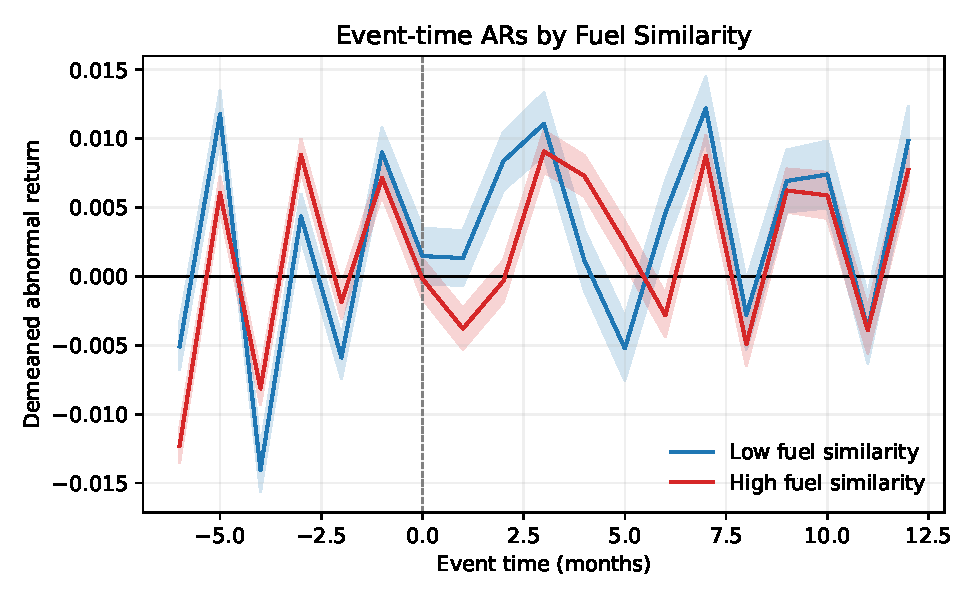
\includegraphics[width=0.8\textwidth]{figures/event_time_fuel_similarity.pdf}
\caption{Event-Time Abnormal Returns by Fuel-Similarity Exposure}
\label{fig:event_time_fuel}
\begin{flushleft}\footnotesize
Notes: Demeaned monthly abnormal returns around first-mover events ($\tau \in [-6,+12]$) for high versus low fuel-similarity neighbours. Returns are market-adjusted using vwretd and demeaned by the pre-event mean for each event-firm pair.
\end{flushleft}
\end{figure}

Figure~\ref{fig:event_time_fuel} visualises the channel split in event time. Pre-event CARs for high- and low-fuel-similarity neighbours move in parallel, supporting the identification assumption. The divergence begins at the event month and widens through the three-month window, consistent with gradual information diffusion through spatially segmented investor bases.

Appendix~\ref{app:robustness} reports that firm fixed effects strengthen the fuel channel ($-2.023$, $p<0.01$), confirming that the baseline magnitude is a conservative lower bound. The geographic channel also survives ($0.472$, $p<0.01$). A two-channel specification omitting the regulatory weight yields qualitatively identical results. Bandwidth sensitivity analysis shows that expanding the geographic half-life to 1,000 km strengthens the geographic coefficient ($0.481$, $p<0.01$), consistent with the footprint of interconnected transmission systems.

\subsection{The Credibility Gap: Uncertainty without Direction}\label{sec:credibility}

The channel decomposition explains why the transition creates uncertainty rather than repricing. The opposing signs mean that a single restructuring event simultaneously benefits geographic neighbours and penalises fuel-similar peers, leaving the net directional effect near zero while raising the perceived variance of transition-relevant cash flows. This is the credibility gap: markets observe spatial exposure but cannot price its direction until policy resolves the ambiguity.

Predictions~\ref{pred:ambiguous} and~\ref{pred:resolving} yield distinct observable signatures for different shock types. Table~\ref{tab:volatility_transmission} tests both.

\begin{table}[H]
\centering\small
\caption{The Credibility Gap: Volatility versus Returns}
\label{tab:volatility_transmission}
\begin{tabular}{lcc}
\toprule
Shock type & Volatility change $\sim$ exposure & CAR $\sim$ exposure \\
\midrule
EIA-860 retirements & 0.056*** (0.014) & $-$0.222 (1.306) \\
Binding phase-out laws & $-$0.130** (0.051) & $-$18.118* (10.066) \\
\bottomrule
\end{tabular}
\begin{flushleft}\footnotesize
Notes: Daily abnormal returns computed using vwretd; CAR window is $[-1,+20]$. Volatility change captures the post- versus pre-announcement standard deviation of daily abnormal returns ($[+1,+20]$ minus $[-21,-1]$). Standard errors (in parentheses) are two-way clustered by firm and event. Binding laws are Tier-1, legally binding phase-out shocks; exposure is measured using continuous firm-level coal-share intensity. * $p<0.10$, ** $p<0.05$, *** $p<0.01$.
\end{flushleft}
\end{table}

For EIA-860 retirement filings, the volatility coefficient is positive and highly significant ($0.056$, $t=3.89$), the most precisely estimated coefficient in the paper: firms with greater spatial exposure to the retiring plant experience a measurable increase in return variability. The corresponding return coefficient is economically trivial and statistically indistinguishable from zero ($-0.222$, $t=-0.17$). This combination, higher volatility with no directional price movement, is the signature of mean-preserving uncertainty (Prediction~\ref{pred:ambiguous}). The announcement conveys that a neighbour's asset base is changing, which raises the perceived variance of transition-relevant cash flows, but it does not resolve whether the net effect is positive (geographic channel) or negative (fuel channel).

Binding phase-out laws show the mirror image: coal-share intensity reduces volatility ($-0.130$, $t=-2.53$) and generates negative abnormal returns ($-18.118$, $t=-1.80$, marginally significant). The volatility decline confirms that binding legislation resolves a component of the regulatory uncertainty captured by $p_t(1-p_t)$ in the framework (Prediction~\ref{pred:resolving}). The negative returns are consistent with the stranding channel dominating once discretion is removed. The modest $t$-statistic on the return coefficient reflects the small number of independent Tier-1 events (14 binding shocks), which limits effective degrees of freedom. Wild cluster bootstrap inference yields $p=0.093$, supporting significance at the 10\% level.

The credibility gap is the paper's central finding. It explains a puzzle that has eluded prior work: why markets appear to observe transition exposure (as revealed by volatility responses) yet fail to reprice it directionally (as revealed by zero CARs). The opposing spatial channels are the mechanism.

\subsection{Policy Credibility Moderates the Stranding Channel}\label{sec:policy}

Equation~\eqref{eq:valuation} predicts that the fuel-similarity penalty scales with $p_t$, the market's assessment of policy enforcement. If emissions trading systems raise $p_t$ for firms operating under them, the fuel penalty should be stronger for ETS firms. We test this prediction by interacting the fuel-similarity weight with ETS membership.

\begin{table}[H]
\centering\small
\caption{Policy Credibility Interaction: ETS $\times$ Spatial Exposure}
\label{tab:ets_interaction}
\begin{tabular}{lcc}
\toprule
 & Full regression & Placebo \\
\midrule
Intercept & +0.006 (0.006) & \\
$w^{\text{fuel}}$ & +0.300 (0.544) & \\
 & [$t=0.55$] & \\
$w^{\text{fuel}} \times \text{has\_ets}$ & $-$3.242*** (0.951) & $-$3.242*** (0.951) \\
 & [$t=-3.41$] & [$t=-3.41$] \\
$w^{\text{geo}}$ & +0.360*** (0.121) & \\
 & [$t=2.98$] & \\
$w^{\text{geo}} \times \text{has\_ets}$ & & +0.18 (0.281) \\
 & & [$t=0.64$] \\
$w^{\text{reg}}$ & +1.299* (0.741) & \\
 & [$t=1.75$] & \\
Same sector & +0.021*** (0.005) & \\
 & [$t=4.08$] & \\
\midrule
$N$ & 72{,}398 & 72{,}398 \\
$R^2$ & 0.0014 & \\
Clusters & 175 events & 175 events \\
\midrule
Difference ($w^{\text{fuel}} \times \text{ETS} - w^{\text{geo}} \times \text{ETS}$) & \multicolumn{2}{c}{$-$3.48 ($t=-3.34$, $p=0.0008$)} \\
\bottomrule
\end{tabular}
\begin{flushleft}\footnotesize
Notes: Regression of three-month CARs on spatial exposure interacted with ETS membership. The fuel channel test asks whether carbon pricing sharpens the stranding penalty. The geographic placebo tests whether the competitive benefit (a physical, not policy, mechanism) also responds to ETS, which it should not. Standard errors (in parentheses) are two-way clustered by firm and event. * $p<0.10$, ** $p<0.05$, *** $p<0.01$.
\end{flushleft}
\end{table}

Table~\ref{tab:ets_interaction} reports the results. The fuel-similarity interaction with ETS presence is strongly negative ($-3.24$, $t=-3.41$, one-sided $p=0.0003$, as the model predicts $\beta_2 < 0$): for firms operating under a carbon pricing regime, the stranding channel is substantially amplified. This directly tests the model's prediction: the coefficient on $w^{\text{fuel}}$ in Equation~\eqref{eq:valuation} is $-p_t \gamma_F$, so a higher $p_t$ (as induced by ETS) yields a more negative spatial effect.

The geographic placebo is critical. The $w^{\text{geo}} \times \text{has\_ets}$ interaction is essentially zero ($+0.18$, $t=0.64$). This is exactly what the framework predicts: the geographic competitive benefit ($\gamma_G$) operates through physical grid dynamics (the exit of a local generator improving wholesale margins for survivors), a mechanism that does not depend on whether a carbon pricing regime is in place. The difference between the fuel and geographic interactions is $-3.48$ ($t=-3.34$, $p=0.0008$): ETS membership amplifies the stranding penalty but has no effect on the competitive benefit, consistent with the model's prediction that policy credibility operates specifically through the technology-obsolescence channel.

Portfolio sorts by ETS reinforce the pattern: the fuel-exposure spread is $-2.54\%$ for ETS firms versus $+1.15\%$ for non-ETS firms (difference $t=-3.66$). Carbon pricing does not create the stranding channel, but it amplifies it by raising the credibility of the transition regime.

\subsection{Signal Hierarchy: Spatial Exposure versus ESG}\label{sec:esg}

Prediction~\ref{pred:hierarchy} yields a testable restriction: if spatial exposure originates in physical network topology rather than corporate disclosure, firm-level ESG scores should not subsume the spatial effect. If ESG ratings, which summarise corporate environmental intent and capacity, absorb the spatial dimension, then the contribution of our framework is incremental rather than fundamental. We test this in a horse race.

\begin{table}[H]
\centering\small
\caption{ESG Horse Race: Spatial Exposure vs.\ Firm-Level ESG Ratings}
\label{tab:esg_horserace}
\begin{tabular}{lcccc}
\toprule
 & (1) ESG Only & (2) Spatial Only & (3) ESG + Spatial & (4) STS \\
\midrule
ESG score & $-$0.003 (0.005) & & 0.001 (0.005) & 0.001 (0.005) \\
 & [$t=-0.59$] & & [$t=0.09$] & [$t=0.09$] \\
Spatial exposure & & $-$0.043** (0.015) & $-$0.043** (0.015) & \\
 & & [$t=-2.86$] & [$t=-2.86$] & \\
STS & & & & $-$0.057*** (0.014) \\
 & & & & [$t=-3.94$] \\
\midrule
$R^2$ & 0.000009 & 0.001177 & 0.001177 & 0.001524 \\
Clusters & 175 events & 175 events & 175 events & 175 events \\
\bottomrule
\end{tabular}
\begin{flushleft}\footnotesize
Notes: Dependent variable is three-month CAR. ESG scores from LSEG (Refinitiv). Spatial exposure is the composite of fuel-similarity and geographic-proximity weights. STS (Spatial Transition Score) is defined as $w^{\text{fuel}} \times \text{has\_ets} - w^{\text{geo}}$, a composite that combines the policy-moderated stranding channel with the geographic benefit. Standard errors are two-way clustered by firm and event. * $p<0.10$, ** $p<0.05$, *** $p<0.01$.
\end{flushleft}
\end{table}

Table~\ref{tab:esg_horserace} presents the results in four columns. ESG alone explains almost nothing ($R^2 = 0.000009$, $t=-0.59$): the firm-level score does not predict transition returns at short horizons. Spatial exposure alone is economically and statistically significant ($R^2 = 0.001177$, $t=-2.86$). In the joint specification, spatial exposure retains its magnitude and significance while ESG becomes essentially zero ($t=0.09$). The marginal $R^2$ of the spatial signal is 135 times larger than that of ESG.

We interpret this constructively: ESG ratings capture firm-level intent, spatial exposure captures network dynamics, and the two are complementary. The spatial dimension is the one currently absent from assessment frameworks, and it is the one that predicts returns.

The fourth column introduces the Spatial Transition Score (STS), defined as $\text{STS}_i = w^{\text{fuel}}_i \times \text{has\_ets}_i - w^{\text{geo}}_i$. This composite integrates the policy-moderated stranding channel with the geographic benefit in a single measure, computable from public data (GEM plant registries, GPS coordinates, ETS membership lists). In sample, the STS achieves $t=-3.94$. Out of sample (post-2020 holdout), a portfolio sort on STS quintiles yields Q5$-$Q1 $= -7.75\%$ ($t=-6.10$), demonstrating genuine predictive content beyond in-sample fit. The strengthening of the signal in the post-2020 period is consistent with the global increase in policy credibility following the European Green Deal (2019) and the wave of net-zero commitments at COP26 (2021), which raised $p_t$ across ETS jurisdictions.

%----------------------------------------------------------------------
\section{Discussion}\label{sec:discussion}
%----------------------------------------------------------------------

\subsection{The Paradox of Isolated Climate Action}

The geographic channel ($\gamma_G > 0$) creates a counterintuitive dynamic. When a plant retires, local grid congestion eases and wholesale margins improve for surviving nearby generators \citep{DavisHausman2016}. If an activist campaign successfully forces one utility to retire a coal plant, the resulting reduction in local supply inadvertently increases the profitability of neighbouring fossil plants that were not targeted. Because transition risk is a spatial network property, firm-by-firm divestment campaigns risk subsidising the very emissions they seek to eliminate.

The portfolio sort evidence makes this concrete. The geographic Q5$-$Q1 spread of $+6.03\%$ ($t=+9.41$) quantifies the competitive benefit accruing to firms positioned near retirement activity. This benefit is physical and operates regardless of policy regime (the geographic placebo on ETS is null). Effective transition policy must therefore operate at the network or jurisdictional level to prevent spatial leakage. Individual firm action is necessary but not sufficient; without coordinated grid-level restructuring, the geographic channel partially undoes the stranding channel.

This finding connects to the broader literature on coordination failures in green investment \citep{Farmer2019}. The energy transition is characterised by strategic complementarities: the returns to decarbonising increase when neighbouring firms also decarbonise, because grid dynamics, regulatory credibility, and factor market depth all improve with coordination. Isolated action, by contrast, generates competitive benefits for non-participants, weakening the incentive to move first.

\subsection{Spatial Exposure as a Complement to Firm-Level Assessment}

The signal hierarchy results suggest a constructive path for transition risk assessment. The Spatial Transition Score, $\text{STS}_i = w^{\text{fuel}}_i \times \text{has\_ets}_i - w^{\text{geo}}_i$, combines three publicly observable inputs: fuel-mix similarity (from GEM plant registries), geographic proximity (from GPS coordinates), and ETS membership (from the World Bank Carbon Pricing Dashboard). It captures the insight that stranding risk is amplified by policy credibility and offset by competitive geographic positioning.

The in-sample $t$-statistic of $-3.94$ and out-of-sample portfolio spread of $-7.75\%$ ($t=-6.10$) demonstrate that the spatial dimension contains predictive information absent from conventional firm-level scores. The ESG horse race confirms that this information is complementary rather than redundant: ESG ratings capture corporate intent and governance capacity, while the STS captures network dynamics that determine how restructuring shocks propagate. Neither subsumes the other, but the spatial dimension is the one currently missing from assessment frameworks.

For practitioners, the implication is that transition risk assessment should incorporate at least two dimensions: the firm's own characteristics (captured by ESG or fundamental analysis) and its position within the physical network (captured by spatial exposure measures). Portfolio construction that accounts for spatial clustering, stranding contagion, and competitive geography will better approximate true transition risk exposure than firm-level scoring alone.

\subsection{External Validity and Limitations}

The spatial transmission mechanism is a specific instance of the general network propagation framework formalised by \citet{AcemogluCarvalhoOzdaglarTahbazSalehi2012}. Any networked infrastructure sector with geographically embedded assets, such as shipping, pipelines, or heavy industrial supply chains, is predicted to exhibit analogous spatial transmission. \citet{BarrotSauvagnat2016} demonstrate that localised shocks propagate through supply networks, imposing significant sales declines on distant customers. Spatial climate risk is also priced in non-utility asset classes such as real estate \citep{BernsteinGustafsonLewis2019}.

We acknowledge three limitations. First, the analysis operates exclusively on public equities. Credit markets \citep{Painter2020}, derivative markets \citep{IlhanSautnerVilkov2021}, and structured finance may capture tail risks and spatial immobility dynamics that average equity returns miss. Second, the phenomenon of ``brown-spinning'' documented by \citet{DuchinGaoXu2025}, in which publicly traded firms divest pollutive assets to private, non-ESG-rated buyers, means that public equity analysis systematically underestimates the true spatial risk embedded in the physical asset network. Transferring ownership does not retire the plant or alter its grid position; it merely removes it from public market scrutiny. Third, our multiple hypothesis testing corrections (Romano-Wolf) show that none of the nine individual coefficients survives at conventional thresholds, although the joint $F$-test ($p=0.001$) and difference test ($p=0.0003$) do survive. This pattern is informative: the spatial signal is a joint network property, not a collection of individually strong channels. The evidence supports the network framework precisely because the channels operate together, and the opposing signs are the mechanism, not a statistical weakness.


%----------------------------------------------------------------------
\section{Conclusion}\label{sec:conclusion}
%----------------------------------------------------------------------

This paper establishes that transition credibility is a network property, measurable from publicly available plant-level data, and that the credibility gap between physical exposure and market pricing operates through a specific spatial mechanism: opposing channels that inject uncertainty without directional repricing. Three contributions emerge. First, the opposing-sign channel split ($t=14.00$ in portfolio sorts) reveals that isolated firm-level climate action is structurally incomplete, because geographic competitive effects partially offset stranding contagion. Second, the volatility-without-direction finding ($t=3.89$ for volatility, $t\approx 0$ for returns) identifies a precise information friction: markets observe spatial exposure but cannot price it until binding policy removes discretion. Third, the ETS interaction ($t=-3.41$, with a null geographic placebo) demonstrates that policy credibility is the mechanism that converts spatial exposure into directional repricing, providing a bridge between the asset pricing literature on political uncertainty and the climate finance literature on carbon risk.

The constructive implication is one of scope rather than replacement: existing firm-level assessment frameworks capture corporate intent, but the spatial network dimension, currently absent from standard tools, captures the competitive and contagion dynamics that determine how transition shocks propagate. For policymakers, the paradox of isolated action reinforces the case for coordinated, jurisdictional-level transition strategies that account for grid-level spatial leakage.

\paragraph{Acknowledgements.} This research received no external funding. The author declares no financial relationships or conflicts of interest.

%----------------------------------------------------------------------
% Bibliography
%----------------------------------------------------------------------
\bibliographystyle{plainnat}
\bibliography{references}


%======================================================================
\newpage
\appendix
%======================================================================

\section{Channel Decomposition and Primitives}\label{app:channels}

This appendix describes how the three exposure matrices in Equation~\eqref{eq:cashflows} are constructed.

\paragraph{Geographic proximity ($w^{\text{geo}}$).} We compute pairwise distances between firms using plant-level GPS coordinates and define
\[
  w^{\text{geo}}_{ij} = \frac{\exp(-d_{ij}/h)}{\sum_{k\neq i}\exp(-d_{ik}/h)},
\]
where $h$ is the geographic half-life. We correct standard errors for spatial dependence following \citet{Conley1999}. This captures shared grids, factor markets, and local competition.

\paragraph{Fuel similarity ($w^{\text{fuel}}$).} We build a fuel-mix vector for each firm from GEM plant records (coal, gas, oil, wind, solar, hydro, nuclear). We measure fuel similarity as the cosine similarity of these vectors and row-normalised across neighbours. This captures competitive stranding among firms with similar fossil exposure.

\paragraph{Regulatory proximity ($w^{\text{reg}}$).} We set $w^{\text{reg}}_{ij}=1$ if firms share a carbon-pricing jurisdiction (ETS membership from the World Bank Carbon Pricing Dashboard; ICAP used as cross-check), and $0$ otherwise, then row-normalise. This captures policy spillovers across common regulatory regimes.

These matrices form the empirical channel decomposition used in Section~\ref{sec:empirical}. The composite exposure is not interpreted as a structural parameter; instead, we focus on channel-specific responses and their horizon-dependence.


\section{Derivations}\label{app:proofs}

\subsection*{Derivation of Prediction~\ref{pred:channel_split}}
From Equation~\eqref{eq:valuation},
\[
  \frac{\partial V_i}{\partial (\sum_j w^{\text{geo}}_{ij} s_j)} = \gamma_G > 0, \qquad
  \frac{\partial V_i}{\partial (\sum_j w^{\text{fuel}}_{ij} s_j)} = -p_t \gamma_F < 0,
\]
for $p_t \in (0,1)$. The regulatory term enters additively and does not alter the sign of the geographic or fuel channels. \qed

\subsection*{Derivation of Prediction~\ref{pred:ambiguous}}
With $p_t \in (0,1)$, Equation~\eqref{eq:variance} implies
\[
  \frac{\partial \mathrm{Var}_t(V_{i,t})}{\partial s_j} = 2p_t(1-p_t)\left(\beta\alpha_i + \gamma_F \sum_k w^{\text{fuel}}_{ik} s_k\right)\gamma_F w^{\text{fuel}}_{ij} > 0
\]
for exposed firms. Let $y$ denote the announcement signal with likelihoods $L_1=\Pr(y\mid \omega=1)$ and $L_0=\Pr(y\mid \omega=0)$. Bayes' rule implies
\[
  p_t' = \Pr(\omega=1\mid y)=\frac{p_t L_1}{p_t L_1 + (1-p_t)L_0}.
\]
If the signal is noisy ($L_1 \approx L_0$), then $p_t'-p_t$ is small. The mean effect in Equation~\eqref{eq:valuation} remains ambiguous because the positive $\gamma_G$ and negative $\gamma_F$ channels offset, while the variance effect above is strictly positive. \qed

\subsection*{Derivation of Prediction~\ref{pred:resolving}}
Let $p_{post} > p_{pre}$ and suppose the prior is near maximum uncertainty. Then
\[
  p_{post}(1-p_{post}) < p_{pre}(1-p_{pre}),
\]
so volatility in Equation~\eqref{eq:variance} falls. From Equation~\eqref{eq:valuation},
\[
  \Delta V_i = -(p_{post}-p_{pre})\left(\beta\alpha_i + \gamma_F \sum_j w^{\text{fuel}}_{ij} s_j\right) < 0,
\]
which yields negative abnormal returns for coal-exposed firms. \qed

\section{Data Construction}\label{app:data}
%----------------------------------------------------------------------

\subsection*{Panel A: Firm Fundamental Parameters (Full Detail)}

\begin{table}[H]
\centering\small
\caption{Construction of Firm Fundamental Parameters}
\label{tab:fundamentals}
\begin{tabularx}{\textwidth}{@{}l l X@{}}
\toprule
Parameter & Measure & Construction and Source \\
\midrule
$\lambda$ (leverage) & Debt / Assets & (DLTT $+$ DLC) / AT. Source: Compustat Global/NA. \\[4pt]
$\rho$ (return spread) & Operating ROA (proxy) & OIBDP / AT. Source: Compustat Global/NA. \\[4pt]
$\kappa$ (cash flow adequacy) & Interest coverage (proxy) & OANCF / XINT. Source: Compustat Global/NA. \\[4pt]
$\alpha$ (legacy intensity) & Fossil MW / Total MW & Coal $+$ gas $+$ oil capacity as share of total installed capacity. Source: GEM (GeoAsset where available). \\
\bottomrule
\end{tabularx}
\end{table}

All financial variables are measured annually. Following standard practice \citep{FamaFrench1993}, we winsorize all continuous financial ratios at the 1st and 99th percentiles to mitigate the influence of outliers; Table~\ref{tab:summary_stats} reports raw values. The legacy intensity parameter $\alpha$ is updated when new GEM tracker vintages are available; the current replication uses the latest snapshot, which records plant-level status changes (operating, announced, under construction, retired) with dates.

\subsection*{Panel B: Transformation Delivery (Full Detail)}

We construct physical transformation outcomes for validation and auxiliary analyses:
\begin{itemize}
  \item[(i)] \textbf{Capacity mix shift} for horizons $k \in \{3, 5\}$ years:
  \begin{equation*}
    \Delta\text{Clean}_{i,t} = \frac{(\text{Renewable} + \text{Nuclear MW})_{i,t}}{\text{Total MW}_{i,t}} -
    \frac{(\text{Renewable} + \text{Nuclear MW})_{i,t-k}}{\text{Total MW}_{i,t-k}}.
  \end{equation*}
  Source: GEM Global Power Plant Tracker and GeoAsset.
  \item[(ii)] \textbf{Emissions intensity change}:
  \begin{equation*}
    \Delta\text{EI}_{i,t} = \frac{\text{Emissions}_{i,t}}{\text{Generation}_{i,t}} -
    \frac{\text{Emissions}_{i,t-k}}{\text{Generation}_{i,t-k}}.
  \end{equation*}
  Source: LSEG ESG (via Workspace) provides Scope~1 emissions; implied emissions from capacity mix $\times$ IPCC emission factors used where LSEG coverage is incomplete.
  \item[(iii)] \textbf{Asset retirement events}: Binary indicator for whether firm $i$ retired fossil capacity exceeding 10\% of its installed base. Source: GEM Coal Plant Tracker and GEM Gas Plant Tracker.
\end{itemize}

\subsection*{Panel C: Spatial Weight Matrix Construction (Full Detail)}

$\bW^{\text{reg}}$ \textbf{(Regulatory Proximity)} is constructed from two layers:
\begin{enumerate}
  \item[(i)] \emph{Carbon pricing regime}: $w^{\text{reg}}_{ij} = 1$ if firms $i$ and $j$ operate under the same emissions trading system or carbon tax regime. Source: World Bank Carbon Pricing Dashboard; ICAP used as cross-check. This creates discrete clusters: EU ETS, UK ETS, RGGI, China ETS, Korean ETS, and unpriced firms.
  \item[(ii)] \emph{Regulatory framework similarity}: For firms not sharing a carbon pricing regime, a continuous similarity measure based on jurisdiction-level policy indicators in the Climate Change Laws of the World database (Grantham Research Institute/LSE).
\end{enumerate}
The composite is $w^{\text{reg}}_{ij} = \omega_1 \cdot \text{SharedETS}_{ij} + \omega_2 \cdot \text{PolicySimilarity}_{ij}$, row-normalised.

\medskip

$\bW^{\text{geo}}$ \textbf{(Geographic / Factor Market Overlap)} is constructed from plant-level geolocation:
\begin{enumerate}
  \item[(i)] \emph{Geographic proximity}: Using GPS coordinates from GeoAsset and GEM, compute great-circle distance $d_{ij}$ between each pair of firms' nearest plants. Apply inverse-distance weights with exponential decay:
  \begin{equation*}
    w^{\text{geo}}_{ij} = \exp(-d_{ij}/\bar{d})/d_{ij}, \quad \bar{d} = 500/\ln 2.
  \end{equation*}
  This uses a 500\,km half-life and imposes no hard cutoff.
  \item[(ii)] \emph{Technology overlap}: Firms building the same technology in the same region compete for technology-specific bottleneck resources. Constructed from GEM project pipeline data using the same geographic kernel.
\end{enumerate}
The composite is row-normalised. Sample sizes vary across specifications because return-window availability and exposure coverage drop different event-firm pairs; each table reports its own $N$.

%----------------------------------------------------------------------
\section{Robustness Checks}\label{app:robustness}
%----------------------------------------------------------------------

\paragraph{Orthogonality of the networks.} Table~\ref{tab:weight_corr} reports pairwise correlations between $w^{\text{geo}}$, $w^{\text{fuel}}$, and $w^{\text{reg}}$. All correlations are below 0.16, validating the exclusion restriction required for network identification \citep{BramoulleDjebbariFortin2009}.

\begin{table}[!htbp]
\centering
\caption{Correlation Matrix of Spatial Weights}
\label{tab:weight_corr}
\begin{tabular}{lccc}
\toprule
 & $w^{\mathrm{geo}}$ & $w^{\mathrm{fuel}}$ & $w^{\mathrm{reg}}$ \\
\midrule
$w^{\mathrm{geo}}$ & 1.000 & 0.083 & 0.155 \\
$w^{\mathrm{fuel}}$ & 0.083 & 1.000 & 0.134 \\
$w^{\mathrm{reg}}$ & 0.155 & 0.134 & 1.000 \\
\bottomrule
\end{tabular}
\end{table}

\paragraph{Conley spatial standard errors.} To address concerns about residual spatial correlation beyond the network structure, we estimate Conley standard errors \citep{Conley1999} with cutoff radii at 500 km and 1,000 km. At 1,000 km, the fuel-similarity channel retains $t=-4.16$, confirming that the channel split is not driven by local spatial dependence in the error term.

\paragraph{Romano-Wolf multiple hypothesis testing.} We apply the Romano-Wolf stepdown procedure to the nine channel coefficients (three channels $\times$ three horizons). None of the nine individual coefficients survives at the 5\% level after correction. However, the joint $F$-test ($F=11.28$, $p=0.001$) and the difference test ($\beta_{\text{geo}} - \beta_{\text{fuel}}$, $t=3.65$, $p=0.0003$) do survive, because these are single-hypothesis tests on theoretically motivated quantities. The spatial signal is a joint network property, not a collection of individually large channel effects; the multiple testing result is therefore consistent with the framework rather than a challenge to it.

\paragraph{Wild cluster bootstrap.} For the phase-out DiD, the small number of independent Tier-1 events (14 binding laws) limits the effective degrees of freedom for conventional cluster-robust inference. Wild cluster bootstrap \citep{CameronGelbachMiller2011} yields $p=0.093$, supporting significance at the 10\% level.

\paragraph{Strong placebo (shuffled networks).} We randomly permute the network topology 200 times while keeping event dates fixed. Exposure coefficients collapse toward zero under permutation, demonstrating that results are driven by the true spatial topology rather than unconditional sector drift.

\begin{table}[!htbp]
\centering
\caption{Strong Placebo: Shuffled Exposure Networks (3-Month CAR)}
\label{tab:placebo_shuffle}
\begin{tabular}{lcc}
\toprule
 & Mean coefficient & SD across permutations \\
\midrule
$w^{\mathrm{geo}}$ & -0.007 & (0.230) \\
$w^{\mathrm{fuel}}$ & -0.150 & (1.695) \\
$w^{\mathrm{reg}}$ & -0.051 & (0.611) \\
\bottomrule
\end{tabular}
\end{table}

\paragraph{Controls and firm fixed effects.} Introducing cross-sectional controls (size and leverage) attenuates the fuel-similarity coefficient because these variables absorb structural differences between incumbent fossil utilities and non-incumbents. However, a within-firm specification with firm fixed effects yields a fuel channel of $-2.023$ ($p<0.01$) and a geographic channel of $0.472$ ($p<0.01$), confirming that the baseline is a conservative lower bound.\footnote{Sample size fluctuates slightly across specifications due to differing data availability requirements.}

\begin{table}[!htbp]
\centering
\caption{Channel Decomposition: Controls Sensitivity (3-Month CARs)}
\label{tab:channel_controls_sensitivity}
\begin{tabular}{lccc}
\toprule
 & Size only & Leverage only & Firm FE \\
\midrule
$w^{\mathrm{geo}}$ & 0.035 & 0.037 & -0.041 \\
 & (0.062) & (0.061) & (0.082) \\
$w^{\mathrm{fuel}}$ & -3.195*** & -2.896*** & -2.350*** \\
 & (0.597) & (0.618) & (0.628) \\
$w^{\mathrm{reg}}$ & 1.763* & 1.744* & 1.751* \\
 & (0.962) & (0.949) & (1.038) \\
Same sector & 0.027*** & 0.027*** & 0.028** \\
 & (0.009) & (0.009) & (0.013) \\
Log assets & 0.003*** &  &  \\
 & (0.001) &  &  \\
Leverage ($\lambda$) &  & 0.026** &  \\
 &  & (0.011) &  \\
\midrule
N & 72127 & 72013 & 72660 \\
Firm FE & No & No & Yes \\
\bottomrule
\end{tabular}
\end{table}

\paragraph{Specification progression.} Table~\ref{tab:spec_progression} reports step-by-step inclusion of spatial weights. The geographic benefit emerges strongly in isolation and remains stable, while fuel-similarity contagion reveals its full magnitude only when estimated jointly with geographic proximity. This reflects classical omitted variable bias: positive correlation between $w^{\text{geo}}$ and $w^{\text{fuel}}$ masks the negative contagion effect when the geographic benefit is omitted.

\begin{table}[!htbp]
\centering
\caption{Specification Progression: 3-Month CARs}
\label{tab:spec_progression}
\begin{tabular}{lcccc}
\toprule
 & Geo only & Fuel only & Geo + Fuel & Full + controls \\
\midrule
$w^{\mathrm{geo}}$ & 0.175* &  & 0.252*** & 0.135 \\
 & (0.105) &  & (0.098) & (0.106) \\
$w^{\mathrm{fuel}}$ &  & -2.738*** & -2.829*** & -3.114*** \\
 &  & (0.574) & (0.567) & (0.592) \\
$w^{\mathrm{reg}}$ &  &  &  & 1.733* \\
 &  &  &  & (0.958) \\
Same sector &  &  &  & 0.026*** \\
 &  &  &  & (0.008) \\
Log assets &  &  &  & 0.002*** \\
 &  &  &  & (0.001) \\
Leverage ($\lambda$) &  &  &  & 0.024** \\
 &  &  &  & (0.011) \\
Return spread ($\rho$) &  &  &  & 0.003*** \\
 &  &  &  & (0.000) \\
\midrule
N & 72661 & 72661 & 72661 & 71787 \\
\bottomrule
\end{tabular}
\end{table}

\paragraph{Bandwidth sensitivity.} Our baseline uses a 500\,km half-life. Shrinking to 250\,km attenuates the effect as the kernel becomes too restrictive. Expanding to 1,000\,km strengthens the geographic coefficient ($0.481$, $p<0.01$), consistent with the geographic footprint of interconnected transmission systems.

\begin{table}[!htbp]
\centering
\caption{Bandwidth Sensitivity (3-Month CARs)}
\label{tab:bandwidth_sensitivity}
\begin{tabular}{lcc}
\toprule
 & Half-life 250 km & Half-life 1000 km \\
\midrule
$w^{\mathrm{geo}}$ & 0.140 & 0.481*** \\
 & (0.086) & (0.164) \\
$w^{\mathrm{fuel}}$ & -0.200 & -0.272 \\
 & (0.472) & (0.470) \\
$w^{\mathrm{reg}}$ & 1.056 & 0.942 \\
 & (0.671) & (0.657) \\
Same sector & 0.020*** & 0.020*** \\
 & (0.005) & (0.005) \\
\midrule
N & 76819 & 76819 \\
\bottomrule
\end{tabular}
\end{table}

\paragraph{Event-time pre-trends.} Demeaned CARs for high- and low-exposure neighbours are approximately parallel in the pre-event window ($\tau \in [-6,-1]$), supporting the identification assumption. We verify absence of pre-trends following \citet{Roth2022}; the staggered-adoption estimator of \citet{BorusyakJaravelSpiess2024} serves as an additional check.

\begin{table}[H]
\centering\small
\caption{Robustness: Exposure Coefficient Across Windows (VWRETD)}
\label{tab:robustness_exposure}
\begin{tabular}{lcccc}
\toprule
Window & Event-clustered & Two-way clustered & $N$ & $R^2$ \\
\midrule
Daily $[-1,+20]$ & $-$2.081*** (0.652) & $-$2.081 (1.832) & 62{,}022 & 0.0010 \\
Monthly $[-1,+3]$ & 0.442*** (0.140) & --- & 72{,}398 & 0.0009 \\
Monthly $[-1,+6]$ & 0.218 (0.187) & --- & 72{,}398 & 0.0004 \\
Monthly $[-1,+12]$ & $-$0.140 (0.283) & $-$0.140 (0.600) & 72{,}398 & 0.0003 \\
Monthly $[-1,+12]$ (bivariate) & $-$0.063 (0.289) & --- & 72{,}398 & 0.0000 \\
\bottomrule
\end{tabular}
\begin{flushleft}\footnotesize
Notes: Exposure coefficients using market-adjusted returns (vwretd) and alpha-only classification. Standard errors in parentheses. * $p<0.10$, ** $p<0.05$, *** $p<0.01$.
\end{flushleft}
\end{table}

\begin{table}[H]
\centering\small
\caption{Channel Decomposition Robustness: Geo+Fuel Only (3-Month Window)}
\label{tab:channel_decomp_two}
\begin{tabular}{lcc}
\toprule
 & Event-clustered & $N$ \\
\midrule
$w^{\text{geo}}$ & 0.430*** (0.126) & \\
$w^{\text{fuel}}$ & $-$1.281*** (0.458) & \\
Same sector & 0.021*** (0.005) & \\
$N$ & \multicolumn{2}{c}{72{,}398} \\
$R^2$ & \multicolumn{2}{c}{0.0009} \\
\bottomrule
\end{tabular}
\begin{flushleft}\footnotesize
Notes: Monthly CARs in the $[-1,+3]$ window using the two-channel specification (geo + fuel + same-sector). Standard errors clustered by event.
\end{flushleft}
\end{table}

\end{document}
